\subsection{Ordinary Differential Equations}
\begin{definition}
	An ordinary differential equation is an equation involving a function of a single variable and its derivatives.
\end{definition}
\begin{example}
	\vspace{-\baselineskip}
	\begin{flalign*}
		& y' = y & \\
		& y' = y^2 - t \\
		& y'' + y' = ye^t
	\end{flalign*}
\end{example}
\subsection{Normal Forms}
\begin{definition}
	A first order equation $y' = f\p{t, y}$ is said to be in normal form. More generally, $y^{(n)} = f\p{t, y^{(1)}, y^{(2)}, \ldots, y^{(n-1)}}$ is in normal form.
\end{definition}
\begin{example}
The normal form of $y' + 2ty = 0$ is given by $y' = -2ty$.
\end{example}
\par\bigskip
Differential equations can have many solutions. In the above equation, all solutions are in the form $y\p{t} = Ce^{-t^2}$, so it is called the \textit{general solution} to the above ODE.
\begin{definition}
	The general solution is the family of solutions depending on some parameters that give all but a finite number of solutions.
\end{definition}

\subsection{Initial Value Problems}
\begin{definition}
	A first order ODE $y' = f\p{t, y}$ together with the initial value $y\p{t_0} = y_0$ is called an initial value problem (\textrm{abbreviated as IVP}).
\end{definition}
A solution to an initial value problem satisfies both the associated ODE and the initial condition.

From the above example, if we had the initial condition $y\p{0} = 2$, then the solution to the initial value problem would be $y\p{t} = 2e^{-t^2}$.

\pagebreak
\subsection{Interval of Existence}
\begin{definition}
	Suppose $y = y\p{t}$ satisfies an initial value problem with initial condition $y\p{t_0} = y_0$. Then the interval of existence is the largest interval containing $t = t_0$ on which $y\p{t}$ is defined.
\end{definition}
\begin{example}
	\vspace{-0.5\baselineskip}
	\begin{flalign*}
		&
		\begin{cases}
			y' = y^2 \\
			y\p{0} = 2
		\end{cases}
		&
	\end{flalign*}
	Solution: $\displaystyle y\p{t} = \frac{1}{\frac{1}{2} - t}$
	
	The interval of existence for this IVP is $\p{-\infty, \, \frac{1}{2}}$ (as opposed to the set $\mathbb{R} - \left\{ \frac{1}{2} \right\}$, which is not connected).
\end{example}

\subsection{Geometric Meaning}
Consider $y' = f\p{t, y}$ with $y\p{t_0} = y_0$. If $y\p{t}$ is a solution to the problem, then for any $t$, we must have $\underbrace{y'\p{t}}_{\mathclap{\substack{\text{Slope of } \\ \text{tangent line at }t.}}} = f\p{t, y\p{t}}$.

\subsection{Direction Fields}
\begin{definition}
	A direction field is a plot of line segments, where each one is centered at a point $\p{t, y}$ whose slope is given by $f\p{t, y}$.
\end{definition}
\textit{Example:} $y' = y$
\par
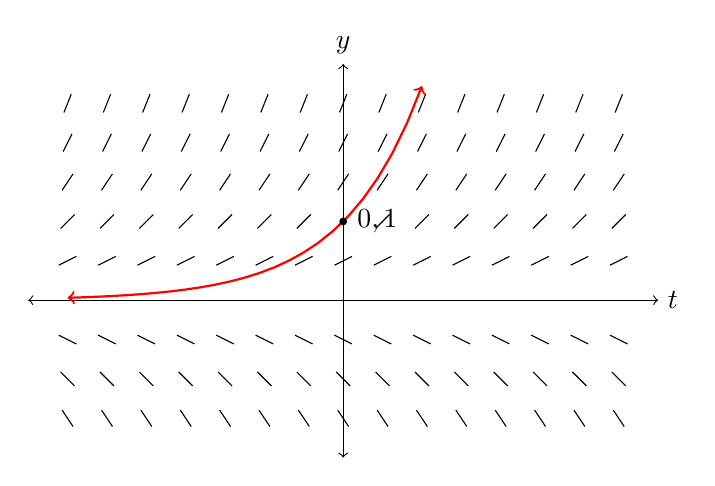
\begin{tikzpicture}
	\draw[<->, black] (-4, 0) -- (4, 0) node[pos = 1, right]{$t$};
	\draw[<->, black] (0, -2) -- (0, 3) node[pos = 1, above]{$y$};
	\foreach \x in {-3.5, -3, ..., 3.5}
		\foreach \y in {-1.5, -1, ..., 2.5}
		{
			\draw[\slopecolor] (\x, \y) -- +({atan(\y)}:-0.125);
			\draw[\slopecolor] (\x, \y) -- +({atan(\y)}:0.125);
		}
	\draw[<->, red, thick, domain = -3.5:1] plot (\x, {exp(\x)});
	\node[circle, inner sep = 1pt, fill = black, label = right:{$\p{0, 1}$}] at (0, 1) {};
\end{tikzpicture}
\par
These are useful for finding numerical solutions to equations we can't solve explicitly.

\subsection{Qualitative Methods}
\textit{Example:} $y' = 1 - y^2$
\par
\begin{figure}[H]
	\begin{minipage}[t]{0.5\textwidth}
		\centering
		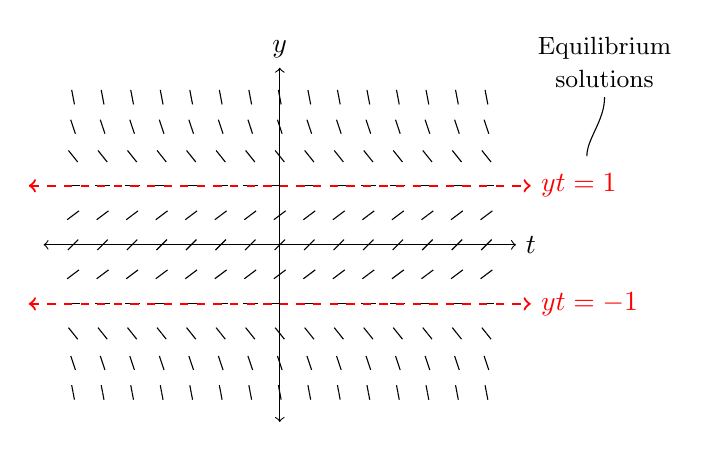
\begin{tikzpicture}[scale = 0.75]
			\draw[<->, black] (-4, 0) -- (4, 0) node[pos = 1, right] {$t$};
			\draw[<->, black] (0, -3) -- (0, 3) node[pos = 1, above] {$y$};
			\foreach \x in {-3.5, -3, ..., 3.5}
				\foreach \y in {-2.5, -2, ..., 2.5}
				{
					\draw[\slopecolor] (\x, \y) -- +({atan(1 - \y * \y)}:-0.125);
					\draw[\slopecolor] (\x, \y) -- +({atan(1 - \y * \y)}:0.125);
				}
			\draw[<->, dashed, thick, red] (-4.25, 1) -- (4.25, 1) node[pos = 1, right] {$y\p{t} = 1$};
			\draw[<->, dashed, thick, red] (-4.25, -1) -- (4.25, -1) node[pos = 1, right] {$y\p{t} = -1$};
			\draw[thin] (5.2, 1.5) .. controls (5.2, 1.8) and (5.5, 2.1) .. (5.5, 2.5) node[pos = 1, above, align = center] {\small Equilibrium \\ \small solutions};
		\end{tikzpicture}
		\caption{Direction Field}
	\end{minipage}%
	\begin{minipage}[t]{0.5\textwidth}
		\centering
		\begin{tikzpicture}[scale = 1.5]
			\draw[<->, black] (-2, 0) -- (2, 0) node[pos = 1, right] {$y$};
			\draw[<->, black] (0, -1.5) -- (0, 1.5) node[pos = 1, above] {$y'$};
			\draw[thin, gray] (-1, -0.25) -- (-1, 0.25) node[pos = 0, below, black] {-1};
			\draw[thin, gray] (1, -0.25) -- (1, 0.25) node[pos = 0, below, black] {1};
			\draw[<->, red, thick] plot[domain = -1.5:1.5] (\x, 1 - \x * \x);
		\end{tikzpicture}
		\caption{Phase Portrait}
	\end{minipage}
\end{figure}
\begin{minipage}[t]{0.5\textwidth}
	Solution classifications:
	\begin{enumerate}[label = \arabic*.]
		\item Equilibrium solution: $y\p{t} = 1$, $y\p{t} = -1$
		\item $\phantom{|} y\p{0} \phantom{|} > 1$: \quad
			\begin{tikzpicture}[scale = 0.35, baseline = -0.8ex]
				\draw[red] (1.25, -0.75) .. controls (-1.3, -0.65) .. (-1.5, 0.5);
			\end{tikzpicture}
		\item $|y\p{0}| < 1$: \quad
			\begin{tikzpicture}[scale = 0.35, baseline = -0.8ex]
				\draw[red] (1.25, 0.5) .. controls (-0.25, 0.5) and (-0.25, -0.75) .. (-1.5, -0.75);
			\end{tikzpicture}
		\item $\phantom{|} y\p{0} \phantom{|} < 1$: \quad
			\begin{tikzpicture}[scale = 0.35, baseline = -0.8ex]
				\draw[red] (1.25, -0.75) .. controls (0.9, 0.5) .. (-1.5, 0.5);
			\end{tikzpicture}
	\end{enumerate}
\end{minipage}%
\begin{minipage}[t]{0.5\textwidth}
	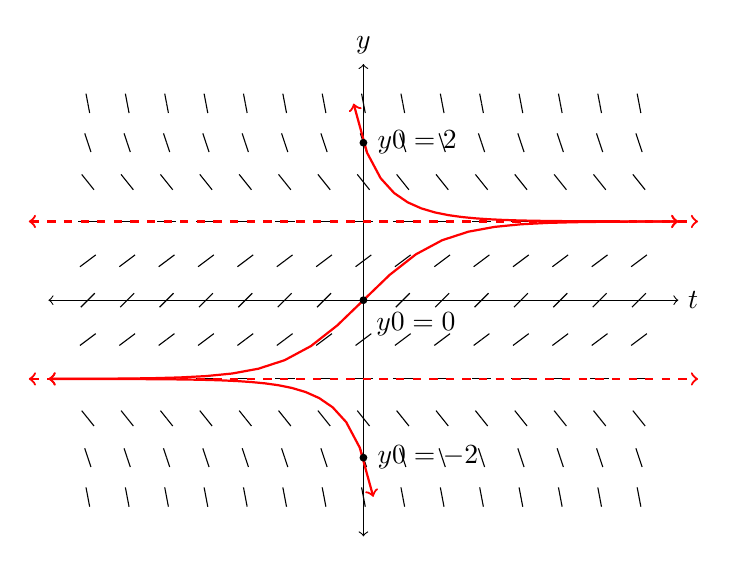
\begin{tikzpicture}[baseline = (current bounding box.north)]
		\draw[<->, black] (-4, 0) -- (4, 0) node[pos = 1, right] {$t$};
		\draw[<->, black] (0, -3) -- (0, 3) node[pos = 1, above] {$y$};
		\foreach \x in {-3.5, -3, ..., 3.5}
			\foreach \y in {-2.5, -2, ..., 2.5}
			{
				\draw[\slopecolor] (\x, \y) -- +({atan(1 - \y * \y)}:-0.125);
				\draw[\slopecolor] (\x, \y) -- +({atan(1 - \y * \y)}:0.125);
			}
		\draw[<->, dashed, thick, red] (-4.25, 1) -- (4.25, 1) node[pos = 1, right] {};
		\draw[<->, dashed, thick, red] (-4.25, -1) -- (4.25, -1) node[pos = 1, right] {};
		\draw[<->, thick, red] plot[domain = -0.125:4] (\x, {(3 * exp(2 * \x) + 1) / (3 * exp(2 * \x) - 1)});
		\node[circle, inner sep = 1pt, fill = black, label = right:{$y\p{0} = 2$}] at (0, 2) {};
		\draw[<->, thick, red] plot[domain = -4:4] (\x, {(exp(2 * \x) - 1) / (exp(2 * \x) + 1)});
		\node[circle, inner sep = 1pt, fill = black, label = below right:{$y\p{0} = 0$}] at (0, 0) {};
		\draw[<->, thick, red] plot[domain = -4:0.125] (\x, {(exp(2 * \x) + 3) / (exp(2 * \x) - 3)});
		\node[circle, inner sep = 1pt, fill = black, label = right:{$y\p{0} = -2$}] at (0, -2) {};
	\end{tikzpicture}
\end{minipage}